\documentclass{article}
\usepackage[utf8]{inputenc}

\usepackage{amsthm}
\usepackage{amsmath}
\usepackage{amssymb}
% Remove line spaces between items of enumerate and itemize
\usepackage{enumitem}
\setlist{noitemsep}
\usepackage{hyperref}
\hypersetup{
	colorlinks=true,
	citecolor=blue,
	urlcolor=blue,
	linkcolor=blue
}
% Math packages
\usepackage{amsthm}
\usepackage{amsmath}
\usepackage{amssymb}

% For more complicated table formatting
\usepackage{multirow}
\usepackage{tabularx}
\newcolumntype{L}[1]{>{\raggedright\let\newline\\\arraybackslash\hspace{0pt}}m{#1}}
\newcolumntype{C}[1]{>{\centering\let\newline\\\arraybackslash\hspace{0pt}}m{#1}}
\newcolumntype{R}[1]{>{\raggedleft\let\newline\\\arraybackslash\hspace{0pt}}m{#1}}

% Remove line spaces between items of enumerate and itemize
\usepackage{enumitem}
\setlist{noitemsep}

% Adds double bracket symbols
\usepackage{stmaryrd}

% Allows to create negation symbols
\usepackage{MnSymbol}

% General math symbols
\DeclareMathOperator{\Id}{Id} % Identity function

% For the little Hasse diagram
\usepackage{tikz}
% LOGIC symbols
% -------------

% Boolean symbols and algebra
\def\Bool{\mathbb{B}}
\def\TRUE{\textsc{true}}
\def\FALSE{\textsc{false}}
\def\AND{\wedge}
\def\bigAND{\bigwedge}
\def\OR{\vee}
\def\bigOR{\bigvee}
\def\NOT{\neg}

% Logical context and related symbols
\def\logCtx{\mathcal{S}}
\def\vstmtSet{\mathcal{S}_\textsf{v}}
\def\dstmtSet{\mathcal{S}_\textsf{d}}
\newcommand{\pAss}[1][\mathcal{S}] {\mathcal{A}_{#1}}
\DeclareMathOperator{\truth}{truth}

% Experimental test symbols
\newcommand{\exptSet}{\mathcal{E}}
\newcommand{\expt}[1][e] {\mathsf{#1}}
\DeclareMathOperator{\result}{result}
\def\SUCCESS{\textsc{success}}
\def\FAILURE{\textsc{failure}}
\def\UNDEF{\textsc{undefined}}

% Statements
\def\tautology{\top} % Tautology
\def\contradiction{\bot} % Contradiction
\newcommand{\stmt}[1][s] {\mathsf{#1}} % Statement
\newcommand{\tstmt}[1][s] {\bar{\mathsf{#1}}} % Theoretical statement

% Relationships between statements
\def\comp{\doublefrown} % Compatibility
\def\ncomp{\ndoublefrown} 
\def\narrower{\preccurlyeq} % Narrowness
\def\nnarrower{\npreccurlyeq}
\def\snarrower{\prec}
\def\nsnarrower{\nprec}
\def\broader{\succcurlyeq} % Broadness
\def\nbroader{\nsucccurlyeq}
\def\sbroader{\succ}
\def\nsbroader{\nsucc}
\def\indep{\upmodels} % Independent
\def\nindep{\nupmodels}

% Experimental domains and related symbols
\newcommand{\edomain}[1][D] {\mathcal{#1}} % Experimental domain
\newcommand{\tdomain}[1][D] {\bar{\mathcal{#1}}} % Theoretical domain
\newcommand{\basis}[1][B] {\mathcal{#1}} % Basis
\newcommand{\resPoss}[1][x] {\mathring{#1}} % Residual possibility
\newcommand{\estPoss}[1][x] {\dot{#1}} % Established possibility

% Formatting for experimental relationships
\newcommand{\erel}[1][r] {#1}

% Formatting for sentence statements
\newcommand{\statement}[1] {\emph{``#1"}}

% Formatting for reference
\newcommand{\refStmt}[1][r]{\textbf{#1}}

\DeclareMathOperator{\ver}{ver}
\DeclareMathOperator{\fal}{fal}
\DeclareMathOperator{\und}{und}

\DeclareMathOperator{\interior}{int}
\DeclareMathOperator{\exterior}{ext}

% Level of detail
\def\eqgran{\doteq}
\def\finer{\leqdot}
\def\nfiner{\nleqdot}
\def\coarser{\geqdot}
\def\sfiner{\lessdot}
\def\scoarser{\gtrdot}

% Theorem styles

%\renewcommand\thesubsection{\thesection.\Alph{subsection}}
%\renewcommand{\theequation}{\thechapter.\arabic{equation}}

\newtheorem{assump}{Assumption}
\renewcommand*{\theassump}{\Roman{assump}}

\newtheorem{axiom}[equation]{Axiom}
\newtheorem{defn}[equation]{Definition}
\newtheorem{prop}[equation]{Proposition}
\newtheorem{coro}[equation]{Corollary}
\newtheorem{thrm}[equation]{Theorem}

%\theoremstyle{definition}

\newenvironment{remark}{\emph{Remark}.}{}
\newenvironment{rationale}{\emph{Rationale}.}{\qed}
\newenvironment{justification}{\emph{Justification}.}{\qed}
\renewenvironment{proof}{\emph{Proof}.}{\qed}



\title{Description granularity: a common foundation for geometry, measures and probability.}
\author{gabriele.carcassi }
\date{September 2020}

\begin{document}

\maketitle

\begin{abstract}
    In this paper we present an order theoretic framework that we hope can be used as a common foundation for geometrical, measure theoretic and probabilistic concepts in the sciences. As in comparative probability, we start with a $\sigma$-complete Boolean algebra that represents all possible descriptions in a given context and impose a preorder. In our case, the preorder does not represent likelyhood comparison, but rather whether one description is at a finer level of granularity than another. At this point, any statement (apart from an impossible one) can be chosen to act as a unit, and a measure (not necessarily bounded) can be constructed to quantify the degree to which the other statements give a more or less refined account. The starting lattice is not necessarily Archimedean, therefore the choice of unit will decide which elements are finite, infinite or infinitesimal. The family of measures so obtained are able to give a size to sets at different level of scale (e.g. points, lines, surfaces, ...) much like geometrical structures do. Our hope is that this structure recovers as special cases the geometrical, measure theoretical and probabilistic constructions we currently use in the sciences while giving a generalization that still works in the case where they fail (e.g. lack of $\sigma$-additivity in quantum probability) or expected to fail (e.g. breakdown at Planck's length).
    
	This work is part of Assumptions of Physics, a project that aims to identify a handful of physical principles from which the basic laws can be rigorously derived  (\url{https://assumptionsofphysics.org}).
\end{abstract}

\def\eqgran{\doteq}
\def\finer{\leqdot}
\def\nfiner{\nleqdot}
\def\coarser{\geqdot}
\def\ncoarser{\ngeqdot}
\def\sfiner{\lessdot}
\def\scoarser{\gtrdot}

\section{Introduction}

This working draft summarizes the status of our work on a new approach to the foundations of geometry and measure theory and is intended to gather early feedback. The goal is to rederive the usual concepts in geometry, measure theory and probability theory from a simpler more general structure. This construction will force us to make explicit the physical requirement that are baked into the use of the common concepts and provide us with a framework that is, hopefully, still valid when those assumptions fail.

The general idea is similar to what is done in comparative probability, yet the techniques extends from a single measure to a family of measure that allow us to define and compare sizes of sets at different scales (e.g. points, lines, surfaces, ...). We start with a $\sigma$-complete Boolean algebra $\tdomain$, a theoretical domain, that represents a set of statements, a set of descriptions, for a physical system in a given context. A Boolean algebra is also a lattice, and therefore already comes equipped with a partial order $\narrower$ such that $\stmt_1 \narrower \stmt_2$ if $\stmt_1 \OR \stmt_2 \equiv \stmt_2$. This partial order indicates whether one statement gives a \textbf{narrower}, more specific, description than the other. For example:
\begin{itemize}
    \item \statement{The position of the object is between 0 and 1 meters} $\narrower$ \statement{The position of the object is between 0 and 1 kilometers}
    \item \statement{The fair dice landed on 1} $\narrower$ \statement{The fair dice landed on 1 or 2}
    \item \statement{The first bit is 0 and the second bit is 2} $\narrower$ \statement{The first bit is 0}
\end{itemize}
In these cases, the first statements has to be ``contained'' in the second, which is more general.

We then suppose we have a way to compare any two statements and decide which one provides a description at a finer level of granularity. This defines an additional preorder $\finer : \tdomain \times \tdomain \to \mathbb{B}$. Saying $\stmt_1 \finer \stmt_2$ means that the description provided by $\stmt_1$ is \textbf{finer}, gives more information, is more precise, than the description provided by $\stmt_2$. For example:
\begin{itemize}
    \item \statement{The position of the object is between 0 and 1 meters} $\finer$ \statement{The position of the object is between 2 and 3 kilometers}
    \item \statement{The fair dice landed on 1} $\finer$ \statement{The fair dice landed on 3 or 4}
    \item \statement{The first bit is 0 and the second bit is 2} $\finer$ \statement{The third bit is 0}
\end{itemize}
In these case, the first statement may not be contained or overlap with the second. Even though the statements come from different disciplines (i.e. geometry, probability and information theory) they all work nicely with the same notion of fineness.

Note that, conceptually, a statement is finer than another if it is true in fewer cases. Therefore the notion of fineness is linked to the notion of ``counting'' of the possible outcomes. It is should be no surprise, then, that the same concept is compatible with the different disciplines above: geometrical size quantifies the ways we can arrange objects; probability theory quantifies the ratio of expected case; information theory needs to quantify the different possible messages stored, computed or transmitted through an information system. Therefore the common structure we propose is not simply a mathematical pattern among disconnected structures: it is a single conceptual framework.

While we borrow many ideas from comparative probability, our goal cannot be achieved with a single measure. A single measure can only compare objects with a finite measure. All objects with zero measure (or infinite measure) are indistinguishable. For example, we want to say:
\begin{itemize}
    \item $\stmt_1$ = \statement{The horizontal position of the object is exactly 0 meter}
    \item $\stmt_2$ = \statement{The horizontal position of the object is exactly 1 or 2 meters}
    \item $\stmt_3$ = \statement{The horizontal position of the object is between 0.5 and 1.5 meters}
    \item $\stmt_4$ = \statement{The horizontal position of the object is between 1.5 and 3.5 meters}
    \item $\stmt_1 \finer \stmt_2 \finer \stmt_3 \finer \stmt_4$
    \item $\stmt_1 \ncoarser \stmt_2 \ncoarser \stmt_3 \ncoarser \stmt_4$
\end{itemize}
Therefore we need to construct a family of measures, each identified by picking a particular statements that acts as a reference, as a unit. This also allows to define more precisely how the physical idea of a unit system can be captured mathematically, something that has never been addressed consistently.

\section{Overview}

We start by giving an overview of the approach. We will give a summary of the main steps and the results, but we will also discuss and justify the starting points and the construction at a physical/conceptual level. It is important for our larger project that the mathematical detail proceeds in lock step with the conceptual and physical understanding. This will allow us in the later section to concentrate on the full  mathematical detail.

We start with a $\sigma$-complete Boolean algebra $\tdomain$, which we call \textbf{theoretical domain}, that can be generated from a countable subset, a countable basis. Conceptually, this represents all the statements that can be associated with an experimental verification procedure. The full detail of why this is the correct abstraction is discussed in detail in our previous work.[TODO: cite book] It is a property of this type of spaces that each statement $\stmt \in \tdomain$ can be expressed as a disjunction of possible cases, of the  \textbf{possibilities} of the domain. Formally, each possibility is minterm of the countable basis.\footnote{The theoretical domain can then be re-expressed as a $\sigma$-algebra one would use in probability theory: a sample space (i.e. the set of possibilities) and a set of events (i.e. the statements in the domain). The advantage of our ``pointless'' constructions is that we can treat domains, subdomains and composite domains in the same manner.}

A Boolean algebra is also a lattice, and therefore $\tdomain$ already comes with a partial order $\narrower$ such that $\stmt_1 \narrower \stmt_2$ if $\stmt_1 \OR \stmt_2 \equiv \stmt_2$. We call \textbf{narrowness} this partial order as it describes whether a statement gives a narrower description of another as we saw in the introduction. The narrowest statement in the domain is the impossibility $\impossibility$ and the broadest one is the certainty $\certainty$.

Conceptually, narrowness allows us to say that a description is more refined than another only if it is fully contained by another. It cannot compare descriptions that do not overlap, that are incompatible. That is why it is not sufficient to quantify the level of description. The ability to compare the granularity of the description of two statements, therefore, is captured by an additional binary relationship $\finer$ we call \textbf{fineness}. To properly capture this idea, finesses must have at least three property.

As we saw, a description is finer than another if it can be true in fewer cases. This intuitive notion is in general ill-defined except than in two cases. A certainties $\certainty$ (e.g. \statement{the position is between minus infinity and plus infinity}) is true in all cases, therefore it must be the coarsest statement. An impossibility (e.g. \statement{the position is between 0 and 1 and also between 2 and 3}) is false in all all cases, therefore it must be the finest statement. This means that fineness must be uniquely bound by the impossibility and the certainty. Any contingent statement must be strictly between the two since there are some cases in which it will be true and others in which it will be false. This is the first required property.

Additionally, if $\stmt_1$ gives finer description than $\stmt_2$ and $\stmt_2$ gives a finer description than $\stmt_3$ then it must be that $\stmt_1$ gives a finer description than $\stmt_3$. This means that fineness is transitive, and this is the second required property.

Lastly, fineness must be related to narrowness: if we have a description that is strictly narrower than another, we expect it to be strictly finer as well. It turns out\cite{definetti} that a single property is enough to specify the relationship. Suppose we have two descriptions $\stmt_1$ and $\stmt_2$ and we pick a third description $\stmt$ that is incompatible with both. By incompatible we mean that two statements can't be both true at the same time (i.e. their conjunction $\stmt_1 \AND \stmt \equiv \impossibility$ is impossible). The respective disjunctions $\stmt_1 \OR \stmt$ and $\stmt_2 \OR \stmt$ will be respectively ``equally'' broader than the respective original statement. Therefore we will want them to be ``equally'' coarser as well. Therefore it must be that $\stmt_1 \finer \stmt$ if and only if $\stmt_2 \finer \stmt$. In other words, fineness must be invariant under addition\footnote{Some authors call this property ``monotony'', which we don't find descriptive. In measure theory, union of disjoint sets plays the role of addition and, in our framework, disjunction of incompatible statements plays the same role.} and this is the third and last required property.

From these starting points one can define and prove a series of useful properties. Most importantly, that fineness is a preorder and that it is monotonic with respect to narrowness. However, these properties will not be enough to recover a unique quantifiable concept of size. To do so, we will require two additional properties which are not strictly a property of fineness itself but a property of the domain. That is, fineness happen to have that property for that specific set of statements but it is not in general true.

We say a theoretical domain $\tdomain$ is uniform if all possibilities are equigranular: they provide the same level of description.\footnote{This plays a role similar to the principle of indifference in classical probability, but does not suffer the same problems.} This is cannot be true for all domains since we can create domains whose possibilities are less refined. Suppose we have a uniform domain with three possibilities: red, green, blue. We can take a ``color bline'' subdomain that cannot distinguish between red an green. This would have two possibilities: red/green and blue. This will not be uniform. The idea is that a uniform domain is a what we want since all cases give us the same level of description. If that's not the case, it's because we are ``missing'' something and we would need to find out what. Uniformity is the first additional property.

We say a theoretical domain $\tdomain$ is totally comparable, or total, if fineness is a total preorder: given any two statements, one is always finer than the other. While this may seem like a reasonable and desirable property, it is actually not always the case. There is no sense, for example, that a range of positions is bigger or smaller than a range of mass or energy. On a symplectic manifold, for example, we can compare areas to each other, yet we cannot compare lengths. In general, the fact that fineness is not total may actually allow us to properly define mathematically the idea of physical dimension. However, for symplicity, in this paper we will concentrate on domains that are totally comparable, leaving the other case for future work.

At this point, we pick a unit $\stmt[u]$ and attempt to construct a unique measure on the sub-algebra of all statements narrower than $\stmt[u]$. One problem is that $\tdomain$ is not in general Archemedian: we are going to have statements that are ``infinitely smaller'' than $\stmt[u]$. In [XXX] we define what it means for a statement to be infinitesimal with respect to another. We then define an equivalence relationship $\equ$ such that two statements are equal in $\stmt[u]$ if they are equigranular up to an infinitesimal of $\stmt[u]$. We then collapse the fineness preorder with that equivalence relationship, and obtain a new preorder $\lequ$. At this point we can show that there exists a unique measure $\mu_{\stmt[u]}$ such that $\mu_{\stmt[u]}(\stmt[u])=1$ and $\mu_{\stmt[u]}(\stmt_1) \leq \mu_{\stmt[u]}(\stmt_2)$ if and only if  $\stmt_1 \lequ \stmt_2$. Since we are restricting ourselves to all statements narrower than $\stmt[u]$, the measure we find is a measure bounded at one, which means we can essentially reuse the techniques from comparative probability even though the context is different.



\begin{enumerate}
    \item Show that if we pick a unit $\stmt[u]$, we can construct a unique measure on the sub-algebra of all statements narrower than $\stmt[u]$. The idea is to define an ordering $\leq_{\stmt[u]}$ that ``squashes" all ``small'' statements to the same equivalence class in $=_{\stmt[u]}$ of the impossibility. An open problem is to understand how to identify the measure zero sets. 
    \item Prove that if $\stmt[v] \narrower \stmt[u]$ then $\mu_{\stmt[u]}(\stmt[w]) = \mu_{\stmt[u]}(\stmt[v]) \mu_{\stmt[v]}(\stmt[w]) $ for all $\stmt[w] \narrower \stmt[v]$. Note that, once this is proven, it tells us that measure zero sets in $\stmt[u]$ are exactly the measure zero sets in $\stmt[v]$.
    \item Given two statements $\stmt[u] \narrower \stmt[v]$, we extend the measure on $\stmt[u]$ by defining $\mu_{\stmt[u]}(\stmt[v]) = 1/ \mu_{\stmt[v]}(\stmt[u])$. If $\mu_{\stmt[v]}(\stmt[u]) = 0$ then $\mu_{\stmt[u]}(\stmt[v]) = \infty$.
    \item To extend the measure on all other statements. Given two statements $\stmt[v]$ and $\stmt[u]$ we can construct the measure $\mu_{\stmt[u]\OR\stmt[v]}$. We have $\mu_{\stmt[u]}(\stmt[v]) = \mu_{\stmt[u]}(\stmt[u]\OR\stmt[v]) \mu_{\stmt[u]\OR\stmt[v]}(\stmt[v])$.
\end{enumerate}


To recover a measure, the idea is to pick a possible statement $\stmt[u] \in \tdomain$ which serves as a unit and construct a total preorder $\leq_{\stmt[u]}$ over $\tdomain_{\stmt[u]} \subseteq \tdomain$. This preorder will induce to a measure. That is, we will be able to find a unique $\mu_{\stmt[u]} : \tdomain_{\stmt[u]} \to \mathbb{R}$ is such that:
\begin{itemize}
    \item $\mu_{\stmt[u]}(\stmt[u])=1$ 
    \item $\mu_{\stmt[u]}(\stmt_1) \leq \mu_{\stmt[u]}(\stmt_2)$ if and only if  $\stmt_1 \leq_{\stmt[u]} \stmt_2$
    \item given $\stmt_1 \ncomp \stmt_2$ we have $\mu_{\stmt[u]}(\stmt_1 \OR \stmt_2) = \mu_{\stmt[u]}(\stmt_1) + \mu_{\stmt[u]}(\stmt_2)$
\end{itemize}
and .

The total preorder $\leq_{\stmt[u]}$ will need to be compatible with fineness. That is, if $\stmt_1 \finer \stmt_2$ then $\stmt_1 \leq_{\stmt[u]} \stmt_2$. It will not be true that $\stmt_1 \sfiner \stmt_2$ then $\stmt_1 <_{\stmt[u]} \stmt_2$. The converse is not true: there will be statements such that $\stmt_1 \leq_{\stmt[u]} \stmt_2$. The totality also needs to be constructed.

Given a total preorder $\leq_{\stmt[u]}$, we say a statement $\stmt$ is zero-comparable to $\stmt[u]$ if and only if $\impossibility =_{\stmt[u]} \stmt$. If $\certainty =_{\stmt[u]} \certainty \AND \NOT \stmt[u]$ then a $\stmt$ is infinitely-comparable to $\stmt[u]$ if and only if $\certainty =_{\stmt[u]} \stmt$. If $\certainty >_{\stmt[u]} \certainty \AND \NOT \stmt[u]$ then there are no statements infinitely-comparable to $\stmt[u]$. All other statements that are comparable are said finitely comparable. If two statements $\stmt_1$ and $\stmt_2$ have the property that $\stmt_1\AND\stmt_2\equ\impossibility$, we say that the pair of statements is null-compatible. This will be denoted by $\stmt_1\ncomp_{\stmt[u]}\stmt_2$. NOTE: I'm not attached to this terminology; it is just a common concept that deserves a name. 


\section{Current attempt}

\begin{defn}
    A \textbf{theoretical domain} $\tdomain$ is a $\sigma$-complete Boolean algebra that can be generated by a countable subset. We call \textbf{narrowness} the partial order of the algebra, that is $x \narrower y$ when $x \OR y = y$. We say $x \in \tdomain$ is a \textbf{possibility} if it is the immediate successor of the impossibility $\impossibility$. That is, $\impossibility \snarrower x$ and there is no $\stmt \in \tdomain$ such that $\impossibility \snarrower \stmt \snarrower x$.
\end{defn}

The fact that the $\sigma$-algebra is generated by a countable set means it is separable.

As a simplifying hypothesis, we assume fineness is a total preorder.

\begin{defn}\label{fineness}
	 Fineness is a binary relationship $\finer : \tdomain \times \tdomain \to \Bool$ with the following properties:
	\begin{itemize}
		\item unique boundedness: for each contingent statement $\stmt \in \tdomain$ we have $\impossibility \sfiner \stmt \sfiner \certainty$
		\item transitivity: if $\stmt_1 \finer \stmt_2$ and $\stmt_2 \finer \stmt_3$ then $\stmt_1 \finer \stmt_3$
		\item addition invariance?: if $\stmt \ncomp \stmt_1$ and $\stmt \ncomp \stmt_2$ then $\stmt_1 \finer \stmt_2$ if and only if $\stmt \OR \stmt_1 \finer \stmt \OR \stmt_2$.
	\end{itemize}
\end{defn}

\begin{defn}
     Let $\stmt_1, \stmt_2 \in \tdomain$. We say $\stmt_1$ is \textbf{equigranular} to $\stmt_2$ (noted $\stmt_1 \eqgran \stmt_2$) if $\stmt_1 \finer \stmt_2$ and $\stmt_2 \finer \stmt_1$.
\end{defn}

\begin{prop}\label{fineness_properties}
    Fineness obeys the following properties:
    \begin{enumerate}
        \item if $\stmt \ncomp \stmt_1$ and $\stmt \ncomp \stmt_2$ then $\stmt_1 \sfiner \stmt_2$ if and only if $\stmt \OR \stmt_1 \sfiner \stmt \OR \stmt_2$ (these two tell us that monotony can be extend to strict fineness and equigranularity)
        \item if $\stmt \ncomp \stmt_1$ and $\stmt \ncomp \stmt_2$ then $\stmt_1 \eqgran \stmt_2$ if and only if $\stmt \OR \stmt_1 \eqgran \stmt \OR \stmt_2$
        \item if $\stmt_1 \narrower \stmt_2$ then $\stmt_1 \finer \stmt_2$ (these three tell us fineness and narrowness are monotonically ordered)
        \item if $\stmt_1 \snarrower \stmt_2$ then $\stmt_1 \sfiner \stmt_2$
        \item if $\stmt_1 \equiv \stmt_2$ then $\stmt_1 \eqgran \stmt_2$
        \item $\stmt_1 \finer \stmt_2$ if and only if $\stmt_1 \AND \NOT \stmt_2 \finer \stmt_2 \AND \NOT \stmt_1$ (these three tell us the region of overlap does not matter)
        \item $\stmt_1 \sfiner \stmt_2$ if and only if $\stmt_1 \AND \NOT \stmt_2 \sfiner \stmt_2 \AND \NOT \stmt_1$
        \item $\stmt_1 \eqgran \stmt_2$ if and only if $\stmt_1 \AND \NOT \stmt_2 \eqgran \stmt_2 \AND \NOT \stmt_1$
        \item if $\stmt_1 \finer \stmt_2$ then $\NOT \stmt_2 \finer \NOT \stmt_1$ (these two tell us that fineness works well with negation)
        \item if $\stmt_1 \sfiner \stmt_2$ then $\NOT \stmt_2 \sfiner \NOT \stmt_1$
        \item if $\certainty \finer \stmt$ then $\certainty \narrower \stmt$ and therefore $\stmt \equiv \certainty$ (these two tells us that fineness can recover narrowness for certainties and impossibilities)
        \item if $\stmt \finer \impossibility$ then $\stmt \narrower \impossibility$ and therefore $\stmt \equiv \impossibility$
    \end{enumerate}
\end{prop}
\begin{remark}
Everything is proved without using totality, so that (if we remove it) everything follows.
\end{remark}

\begin{proof}
For 1, let $\stmt \ncomp \stmt_1$ and $\stmt \ncomp \stmt_2$. Suppose $\stmt_1 \sfiner \stmt_2$, then $\stmt_1 \finer \stmt_2$ and $\stmt_1 \ncoarser \stmt_2$. By monotony we have $\stmt \OR \stmt_1 \finer \stmt \OR \stmt_2$ and $\stmt \OR \stmt_1 \ncoarser \stmt \OR \stmt_2$. Therefore $\stmt \OR \stmt_1 \sfiner \stmt \OR \stmt_2$. Conversely, if $\stmt \OR \stmt_1 \sfiner \stmt \OR \stmt_2$ then $\stmt \OR \stmt_1 \finer \stmt \OR \stmt_2$ and $\stmt \OR \stmt_1 \ncoarser \stmt \OR \stmt_2$. By monotony $\stmt_1 \finer \stmt_2$ and $\stmt_1 \ncoarser \stmt_2$, which means $\stmt_1 \sfiner \stmt_2$.

For 2, now suppose $\stmt_1 \eqgran \stmt_2$, then $\stmt_1 \finer \stmt_2$ and $\stmt_1 \coarser \stmt_2$. By monotony we have $\stmt \OR \stmt_1 \finer \stmt \OR \stmt_2$ and $\stmt \OR \stmt_1 \coarser \stmt \OR \stmt_2$. Therefore $\stmt \OR \stmt_1 \eqgran \stmt \OR \stmt_2$. Conversely, if $\stmt \OR \stmt_1 \eqgran \stmt \OR \stmt_2$ then $\stmt \OR \stmt_1 \finer \stmt \OR \stmt_2$ and $\stmt \OR \stmt_1 \coarser \stmt \OR \stmt_2$. By monotony $\stmt_1 \finer \stmt_2$ and $\stmt_1 \coarser \stmt_2$, which means $\stmt_1 \eqgran \stmt_2$.

For 3, suppose $\stmt_1 \narrower \stmt_2$. Then $\NOT \stmt_2 \ncomp \stmt_2$ and $\NOT \stmt_2 \ncomp \stmt_1$. Since fineness is uniquely bounded, we have $\NOT \stmt_2 \OR \stmt_1 \finer \certainty$. We have $\certainty \equiv \NOT \stmt_2 \OR \stmt_2 \coarser \NOT \stmt_2 \OR \stmt_1$. By monotony we have $\stmt_2 \coarser \stmt_1$.

For 4, suppose $\stmt_1 \snarrower \stmt_2$. Then $\NOT \stmt_2 \OR \stmt_1$ is a contingent statement and, since fineness is uniquely bounded, $\NOT \stmt_2 \OR \stmt_1 \sfiner \certainty \equiv \NOT \stmt_2 \OR \stmt_2$. By 1 we have $\stmt_1 \sfiner \stmt_2$.

For 5, suppose $\stmt_1 \equiv \stmt_2$. Then $\stmt_1 \narrower \stmt_2$ and $\stmt_2 \narrower \stmt_1$, which means $\stmt_1 \finer \stmt_2$ and $\stmt_1 \finer \stmt_2$ and therefore $\stmt_1 \eqgran \stmt_2$.

For 6, note that $\stmt_1 \equiv (\stmt_1 \AND \NOT \stmt_2) \OR (\stmt_1 \AND \stmt_2)$, $\stmt_2 \equiv (\NOT \stmt_1 \AND \stmt_2) \OR (\stmt_1 \AND \stmt_2)$ with $\stmt_1 \AND \stmt_2 \ncomp \stmt_1 \AND \NOT \stmt_2$ and $\stmt_1 \AND \stmt_2 \ncomp \NOT \stmt_1 \AND \stmt_2$. By monotony, $\stmt_1 \finer \stmt_2$ if and only if $\stmt_1 \AND \NOT \stmt_2 \finer \NOT \stmt_1 \AND \stmt_2$.

For 7 and 8, use 1 and 2 respectively in the final step.

For 9, note that $\stmt_1 \AND \NOT \stmt_2 \equiv (\NOT \stmt_2) \AND \NOT (\NOT \stmt_1)$ while $\NOT \stmt_1 \AND \stmt_2 \equiv \NOT (\NOT \stmt_2) \AND (\NOT \stmt_1)$. We have $\stmt_1 \finer \stmt_2$ if and only if (by 6)  $\stmt_1 \AND \NOT \stmt_2 \finer \NOT \stmt_1 \AND \stmt_2$ if and only if (by the equivalence) $(\NOT \stmt_2) \AND \NOT (\NOT \stmt_1) \finer \NOT (\NOT \stmt_2) \AND (\NOT \stmt_1)$ if and only if (by 6 again) $\NOT \stmt_2 \finer \NOT \stmt_1$.

For 10, use 7 whenever 6 was used.

For 11, suppose $\certainty \finer \stmt$. By unique boundedness, $\stmt$ can neither be contingent nor impossible. Therefore $\stmt$ must be certain.

For 12, suppose $\stmt \finer \impossibility$. By unique boundedness, $\stmt$ can neither be contingent nor certain. Therefore $\stmt$ must be impossible.

\end{proof}

\begin{defn}
    A theoretical domain $\tdomain$ is \textbf{uniform} if fineness has the following additional properties:
    \begin{itemize}
        \item totality: for all $\stmt_1, \stmt_2 \in \tdomain$ either $\stmt_1 \finer \stmt_2$ or $\stmt_2 \finer \stmt_1$
        \item uniformity: all possibilities are equigranular.
    \end{itemize}

\end{defn}

\begin{prop}
    Let $\tdomain$ be uniform. Let $\stmt, \stmt_1 \in \tdomain$ such that $\stmt \snarrower \stmt_1$. Then there exist $\stmt_2 \in \tdomain$ such that $\stmt_2 \narrower \stmt_1$ and $\stmt \eqgran \stmt_2$.
\end{prop}


\section{Notes}

One condition for the measure to be unique given a unit statements is that all points (i.e. possibilities in our framework) are equigranular. In fact, consider a domain with just three points not equigranular to each other, but each finer than the other. We can construct any measure that satisfies the requirement by picking three numbers and assigning them accordingly, since we can't determine ``how bigger'' is one point with respect to the other.

\subsection{Finding a probability measure}

Our first goal is to find a measure which is compatible with the fineness preorder. The idea is that fineness tells us which sets are ``larger" (less precise) than each other, regardless of any overlap.  A measure will quantify this and allow us to assign numbers to the sizes.

The paper \cite{probexistence} seems to be extremely relevant here. The basic idea in this paper is to find necessary and sufficient conditions for the existence of a probability measure on a Boolean algebra (e.g. of subsets of some set) which is compatible with a total pre-order. There are a few points to keep in mind. 

First, we need a \emph{total} pre-order. This means for every pair of elements, one is finer than the other. This is certainly not the case for fineness in general: color and position, for example, cannot be compared. This is the goal of defining the \emph{unit} above. The unit serves as a baseline statement against which others can be compared for fineness. For example, a statement about position singles out length as the dimension to compare, or a statement about numbers of objects specifies ``count" as the dimension to compare (e.g. the discrete unit of number of objects). 

Next, we need the three properties specified in the paper, to be written up later! We are optimistic that these three properties are present in our situation. 

There is one additional caveat. The measure constructed by the main theorem in the above-mentioned paper is always a probability measure. This means the whole space has finite measure. For example, one could put the Lebesgue measure on $(0,1)$ but under a homeomorphism $(0,1)\to\mathbb{R}$ induce a finite (probability) measure on  $\mathbb{R}$. If we chose the full set as a unit, we are exactly looking for a probability measure. If we pick a unit that is not the full set, we can also "constrain" the problem to that subset, so that we still have a probability measure. Then we may be able to "stich together" the measures constructed on all equigranular sets assuming they cover the full space. 

\subsection{Applying results of the paper \cite{villegas}}

In this part, we will assume that $\tdomain_{\stmt[u]}$ is a subset of the theoretical domain, $\stmt[u]\in \tdomain_{\stmt[u]}$ is a distinguished element (we'll refer to it as the \emph{unit} when needed), and there is a total pre-order $\leq_{\stmt[u]}$ defined on $\tdomain_{\stmt[u]}$. We will write $=_{\stmt[u]}$ for $\leq_{\stmt[u]}$ and $\geq_{\stmt[u]}$, and we write $<_{\stmt[u]}$ for $\leq_{\stmt[u]}$ and not $=_{\stmt[u]}$. We will use the word ``equiprobable" for $=_{\stmt[u]}$ since it means something different from equigranular (since $\leq_{\stmt[u]}$ is a different ordering from fineness, even though it will be derived from fineness). We assume $\tdomain_{\stmt[u]}$ is closed under complement and countable union (and hence countable intersection), and that there are two additional elements, $\certainty$ and $\impossibility$, which are maximal and minimal in this ordering, respectively.

\begin{remark}
In defining the subset $\tdomain_{\stmt[u]}$ and the total preorder $\leq_{\stmt[u]}$, we will have to be very careful. We want to ``squash" together all the sets which should be measure zero in this unit (e.g. anything ``lower-dimensional"), ``blow up" all the ``infinite measure" subsets (e.g. ``higher dimensional"), and ensure that everything is compatible under this order, so there can be only one ``type" of property under consideration. 
\end{remark}

We write out the main axioms and statements from \cite{villegas} which interest us in this situation, in the notation established earlier. On page 1789, we have the following:

Axiom of Pre-order:
\begin{itemize}
    \item Totality: If $\stmt_1,\stmt_2\in \tdomain_{\stmt[u]}$, then $\stmt_1 \leq_{\stmt[u]} \stmt_2$ or $\stmt_2\leq_{\stmt[u]} \stmt_1$
    \item Reflexivity: For all statements $\stmt\in \tdomain_{\stmt[u]}$, we have $\stmt\leq_{\stmt[u]}\stmt$
    \item Transitivity: For all statements $\stmt_1,\stmt_2,\stmt_3\in \tdomain_{\stmt[u]}$, if $\stmt_1\leq_{\stmt[u]}\stmt_2$ and $\stmt_2\leq_{\stmt[u]}\stmt_3$, then $\stmt_1\leq_{\stmt[u]}\stmt_3$.
    \item Existence of max and min: We have $\impossibility\leq_{\stmt[u]}\certainty$ and \emph{not} $\certainty\leq_{\stmt[u]}\impossibility$. For all $\stmt\in \tdomain_{\stmt[u]}$ we have $\impossibility\leq_{\stmt[u]}\stmt\leq_{\stmt[u]}\certainty$
\end{itemize}

The above list is simply the requirement that $\leq_{\stmt[u]}$ is a total pre-order and that there are a maximal and minimal element. 


Axiom of Monotony: 
Let $\stmt_1,\stmt_2,\stmt_3,\stmt_4\in \tdomain_{\stmt[u]}$. Assume that $\stmt_1\leq_{\stmt[u]} \stmt_2$, $\stmt_3\leq_{\stmt[u]} \stmt_4$, and $\stmt_2\ncomp \stmt_4$ (i.e. $\stmt_2\AND \stmt_4 =_{\stmt[u]} \impossibility$). Then we have $\stmt_1\OR \stmt_3 \leq_{\stmt[u]} \stmt_2\OR \stmt_4.$

Monotony guarantees that given two incompatible statements, each ``bigger" than another statement, then their disjunction is still bigger than the disjunction of the smaller statements. 

The following are consequences of the two axioms above. Let $\stmt_1,\stmt_2,\stmt_3,\stmt_4\in \tdomain_{\stmt[u]}$.
\begin{itemize}
    \item If $\stmt_1\leq_{\stmt[u]} \stmt_2$ and $\stmt_2<_{\stmt[u]} \stmt_3$, then $\stmt_1<_{\stmt[u]}\stmt_3$. 
    \item If $\stmt_1\narrower \stmt_2$ then $\stmt_1\leq_{\stmt[u]} \stmt_2$
    \item If $\stmt_1\leq_{\stmt[u]} \stmt_2$, $\stmt_3\leq_{\stmt[u]} \stmt_4$, $\stmt_2\leq_{\stmt[u]} \stmt_4$, and $v\leq_{\stmt[u]} \stmt_1$, then $\stmt_2 \AND \NOT \stmt_1 \leq_{\stmt[u]} \stmt_4 \AND \NOT \stmt_3$
    \item If $\stmt_1\leq_{\stmt[u]} \stmt_2$ then $\NOT \stmt_2 \leq_{\stmt[u]}\NOT \stmt_1$
\end{itemize}

Next, we will need a more subtle axiom in order to make sense of infinite combinations of statements. 

\begin{remark}
The \emph{fineness} relation $\finer$ should satisfy all of the axioms of pre-order and the axiom of monotony, except for totality. We restrict to $\tdomain_{\stmt[u]}$ in order to get totality. 
\end{remark}

Axiom of Monotone Continuity:
Let $\{\stmt_i : i\in \mathbb{Z}^+\}$ be a sequence of statements which is monotone increasing with respect to narrowness (containment), and let $\stmt = \cup_i\stmt_i$ be the disjunction. Let $t\in \tdomain_{\stmt[u]}$ such that $\stmt_i\leq_{\stmt[u]} t$ for all $i$. Then $\stmt\leq_{\stmt[u]} t$. 

In other words, an infinite disjunction can only strictly exceed a statement in coarseness if the disjunction of a finite subset of them already exceeds it. Here is an interesting consequence of the combination of the above axioms:

\begin{prop}[Corollary to Lemma 1 in \cite{villegas}]
\label{infinitenull}
Let $\{\stmt_i : i\in \mathbb{Z}^+\}$ be an infinite collection such that $\stmt_i\AND\stmt_j =_{\stmt[u]} \impossibility$ for all $i\neq j$, and $\stmt_i =_{\stmt[u]} \stmt_j$ for all $i,j$. Then it must be the case that $\stmt_i=_{\stmt[u]}\impossibility$ for all $i$. 
\end{prop}
This says that infinite collections of equiprobable statements with null overlaps must be null themselves. 

An \emph{atom} is a statement $\stmt\in S$ such that $\impossibility<_{\stmt[u]}\stmt$ and there does not exist any statement $\stmt_2\in S$ such that $\impossibility<_{\stmt[u]} \stmt_2<_{\stmt[u]} \stmt$. In particular, Theorem 5 in \cite{villegas} \S3 includes the fact that $\tdomain_{\stmt[u]}$ is atomless if and only if every statement can be partitioned into two equiprobable statements. Theorem 3 in \S4 states that if $\tdomain_{\stmt[u]}$ is atomless, then there exists a unique probability measure compatible with $\leq_{\stmt[u]}$, and it is countably additive!

\subsection{Using Monotone Continuity}

The core of the proof of Theorem 3 in Section 4 of \cite{villegas} comes from Theorem 5 (iv) in Section 3. In the terminology of Villegas, a \emph{qualitative probability $\sigma$-algebra} is a $\sigma$-algebra of subsets of a space with an ordering that satisfies the Axiom of Pre-order, the Axiom of Monotony, and the Axiom of Monotone Continuity. We also need the language of \emph{atoms}, defined earlier. We will reproduce some of the ideas in the proofs of these theorems in the language of statements and our theoretical domain, while attempting to keep track of the usages of Monotone Continuity. The hope is that there is a weakened version of the axiom that gets us the desired result, or that we can build the ordering $\leq_{\stmt[u]}$ with Monotone Continuity but it can still distinguish the infinite sets described earlier. 

Let $A$ be a statement in $\tdomain_{\stmt[u]}$ with $A>_{\stmt[u]} \impossibility$. A \emph{minor incomplete partition} of $A$ is a collection $M_A$ of statements with the following properties:
\begin{itemize}
    \item We have $\stmt>_{\stmt[u]}\impossibility$ and $\stmt \narrower A$ for all $\stmt\in M_A$, that is, they are non-null and narrower than $A$
    \item For all $\stmt_1,\stmt_2\in M_A$, we have $\stmt_1\AND\stmt_2 =_{\stmt[u]} \impossibility$, that is, they overlap only on statements ``squashed" to zero. 
    \item The disjunction of $M_A$ is finer than its complement in $A$: $$\bigOR_{\stmt\in M_A}\stmt \finer (A\AND \NOT\bigOR_{\stmt\in M_A}\stmt).$$ This is the condition of being \emph{minor}.
    %UM_A finer than A - UM_A^C
\end{itemize}

It is shown in \cite{villegas} that any (minor) incomplete partition is at most countable (Theorem 3). Rather than give the full proof of this fact, we note that it follows from a large collection of lemmas, the most interesting of which is the following, which we will prove below: 

\begin{prop}[Lemma 1 from \cite{villegas}]
If $\{\stmt[a]_i: i\in I\}$ is an infinite set of statements such that (1) $\stmt[a]_i \AND \stmt[a]_j =_{\stmt[u]}\impossibility$ for all $i\neq j$ and (2) $\stmt[a]_i>_{\stmt[u]}\impossibility$ for all $i$, then the following holds. Given a statement $\stmt>_{\stmt[u]}\impossibility$, only finitely many of the $\stmt[a]_i$'s have $\stmt[a]_i>_{\stmt[u]}\stmt$.  
\end{prop}
\begin{proof}
By way of contradiction, let $\stmt[a]_1,\ldots$ be a sequence of statements violating the conclusion (i.e. infinitely many statements $\stmt[a]_i$ with $\stmt[a]_i>_{\stmt[u]}\stmt>_{\stmt[u]}\impossibility$. Consider the new sequence $$\stmt_i = \bigOR\limits_{n=i}^{\infty}\stmt[a]_n.$$ This sequence is monotonely decreasing to the impossibility in narrowness (and hence in fineness and in $>_{\stmt[u]}$), but we also have $\stmt_i\geq_{\stmt[u]}\stmt$ for all $i$. By monotone continuity (the contrapositive), we have $\stmt[s]\leq_{\stmt[u]}\impossibility$, a contradiction. 
\end{proof}

A quick corollary of this is Proposition \ref{infinitenull}, above. Using minor incomplete partitions, we prove the following. 

\begin{prop}[Theorem 4, \S3 \cite{villegas}]
\label{split}
If there are no atoms, then for every statement $\stmt$ there exist statements $\stmt_1$ and $\stmt_2$ such that: $\stmt_1\ncomp \stmt_2$, $\stmt_1\equ\stmt_2$, and $\stmt_1\OR\stmt_2 = \stmt$. In other words, $\stmt$ can be partitioned into two equiprobable (note: I remember we don't like this word but I don't remember if we replaced it or not) statements. 
\end{prop}
\begin{proof}
Let $S$ be the set of minor incomplete partitions of $\stmt$, and endow it with a partial order by inclusion. Given a totally ordered chain in $S$, its union is still a minor incomplete partition, and is thus an upper bound for the chain. We may apply Zorn's lemma to find a maximal element of $S$, the disjunction of which we call $\stmt_1$. We claim that $\stmt_1$ and $\stmt_2:= \stmt\AND\NOT\stmt_1$ are equiprobable, incompatible statements. Incompatibility is immediate from the definition. For equiprobability, first note that by definition of being a minor incomplete partition we have $\stmt_1\lequ\stmt_2$. Next, if $\stmt[t]_1,\ldots$ is a monotone decreasing (with respect to $\lequ$) sequence of statements $\stmt[t]_n>_{\stmt[u]}\impossibility$ narrower than $\stmt_2$ and converging to a zero-comparable event, we have that $\stmt_1\OR\stmt[t]_n>_{\stmt[u]}\stmt_2\OR\stmt[t]_n$ since $\stmt_1$ is maximal. We needed no atoms in order to guarantee this sequence exists (Lemma 3 in Section 3 of \cite{villegas}). It follows by monotone continuity that $\stmt_1\geq_{\stmt[u]} \stmt_2$. 
\end{proof}

We will also need a few types of \emph{random variables} as defined in \cite{villegas} \S3. Let $A({\stmt[u]}) = \{x \in X : x \comp \stmt[u]\}$ be the set of possibilities associated with $\stmt[u]$. This is a subset of the collection of possibilities which will serve as the ``sample space" after picking a unit $\stmt[u]$.

A \emph{uniform sequence of finitely-valued random variables} is a sequence of functions (random variables in the traditional sense) $X_1,X_2,\ldots: A({\stmt[u]})\to E$ where $E$ is a finite set, with the following property: for all $\{x_1,\ldots,x_n\}\subseteq E$, all the events $$\{p\in A({\stmt[u]}): X_i(p) = x_i, i=1,\ldots,n\}$$
are equiprobable ($\equ$ with each other). 

Notice that monotone continuity allows us to let $n\to\infty$ to define events where the whole sequence is specified with the resulting events all being equiprobable. By Proposition \ref{infinitenull} above, all such events are null.

Building on these sequences of random variables, we will use \emph{uniform random variables} to define probability measures. Let $X:A({\stmt[u]})\to[0,1]$ be a random variable, and let $I$ and $J$ be intervals contained in $[0,1]$. We say $X$ is a uniform random variable if $X^{-1}(I)\lequ X^{-1}(J)$ if and only if $|I|\leq|J|$ for all such $I,J$. 

From Proposition \ref{infinitenull}, $X^{-1}(a)$ is a zero-comparable event for all $a\in[0,1]$, and if $0=a_0<a_1<\cdots<a_n=1$, then $X^{-1}([a_i,a_{i+1}))$ are a finite partition of $\tdomain$. 

Next, we will pull many of the above concepts together to show how we obtain a probability measure on $A({\stmt[u]})$ realized as a function on $\tdomain$ compatible with $\lequ$. 

\begin{prop}\label{uniformexist}
If $\tdomain_{\stmt[u]}$ has no atoms with respect to $\lequ$, then there exists a uniform random variable.
\end{prop}
\begin{proof}
By Proposition \ref{split} we may split any statement into two equiprobable, null-compatible sets. Starting with the statement $\stmt[u]$ (here, the ``universe" which we want to have probability 1), repeatedly divide into two statements in stages. At stage $n$ (starting with $n=0$), we will have statements $\stmt[u]^{(n)}_1,\ldots,\stmt[u]^{(n)}_{2^n}$. Now, take the disjunction of alternating statements in each collection so that there is a ``right" and ``left" (odd and even index) half at each stage. For example, at stage $n=1$, the odd and even halves are simply $\stmt[u]^{(1)}_1$ and $\stmt[u]^{(1)}_2$; at stage $n=2$ we have $\stmt[u]^{(2)}_1\OR\stmt[u]^{(2)}_3$ and $\stmt[u]^{(2)}_2\OR\stmt[u]^{(2)}_4$. 

Define a sequence of random variables $X_n:A(\stmt[u])\to\{0,1\}$ by $X_n(a) = 1$ if and only if $a$ is in the odd half in stage $n$. This gives each $a\in A(\stmt[u])$ a binary ``address". By the construction, it follows that this is a uniform sequence of finitely-valued random variables (defined above). 

Now, we define a uniform random variable $X:A(\stmt[u])\to[0,1]$. For $a\in A(\stmt[u])$, define $X(a) = \sum_{n=1}^{\infty}2^{-n}X_n(a)$. In other words, $X(a)$ is the binary expansion $0.X_1(a)X_2(a)\ldots_2$. 

One can show immediately that $X^{-1}(I)\lequ X^{-1}(J)$ if and only if $|I|\leq |J|$ when $I$ and $J$ have endpoints on numbers with finite binary expansions (since $X_1,\ldots,X_n$ are uniform), and by monotone continuity, the uniformity condition extends to arbitrary intervals in $[0,1]$. 
\end{proof}

Finally, we reach our goal of building a probability measure on $A(\stmt[u])$. 

\begin{prop}
If $\tdomain_{\stmt[u]}$ has no atoms with respect to $\lequ$, then there exists a unique compatible probability measure, and it is countably additive. 
\end{prop}
\begin{proof}
By Propsition \ref{uniformexist}, let $X:POSS_{\stmt[u]}\to[0,1]$ be a uniform random variable.
%Define $F:[0,1]\to\tdomain$ by $F(x) = X^{-1}([0,x])$. It is straightforward to see that $F$ is monotone in $x$ (with respect to $\lequ$), and that if $x_n\to x$, then $\lim_nF(x_n) \equ F(x)$. %Started writing this part from paper, but it is not directly used in construction. Will add details later as needed. 
We claim that for any statement $\stmt\in\tdomain_{\stmt[u]}$, there exists a unique number $p\in[0,1]$ such that $\stmt\equ X^{-1}([0,p])$. Define $P:\tdomain_{\stmt[u]}\to[0,1]$ by $P(\stmt)= p$. This defines a probability measure compatible with $\lequ$. Details forthcoming as needed....
\end{proof}

Ideas involved: Defines a function $X:A(\stmt[u])\to [0,1]$ in a way that is consistent with $\lequ$ by having ``larger" sets of possibilities (i.e. coarser statements) corresponding to larger intervals in $[0,1]$. Then, the measure of any other statement is given by finding an equiprobable statement which is the preimage of $[0,p]$ under $X$ and defining the measure to be $p$.  

Wish: find a way to prove the above statements in an order-theoretic way. In particular, we wish to show that the order type of the equigranular-equivalence classes is equivalent to (a subset of) $\mathbb{R}$. Sufficient conditions to be isomorphic to $\mathbb{R}$ are (1) lacking endpoints (2) complete (i.e. has Least Upper Bound property) (3) has dense countable subset. The use of random variables may be very similar to an approach using order theory. For example, the transition from a uniform sequence of finitely-valued random variables into a (single) uniform random variable makes use of a countable dense subset. 








\subsection{Example with lack of monotonicity}

Consider a Euclidian two dimensional space charted by $\{x,y\}$. Let $U_{i,j}$ be the square in the interval $x \in (i, i+1)$ and $y \in (j, j+1)$. Let $V$ be the vertical (infinite) strip in the interval $x \in (0, 1)$ and $W$ the vertical strip in the interval $x \in (0, 2)$. Define the sequence $W_i = \{ U_{0,0}, U_{1,0}, U_{0,1}, U_{1,1}, U_{0,2}, U_{1,2}, U_{0,3}, U_{1,3}, ... \}$. We have $\bigcup\limits_0^\infty W_i = W$. This means $\bigcup\limits_0^n W\finer V$ for all finite $n$ but $\bigcup\limits_0^\infty W_i = W \coarser V$. 

\subsection{Some thoughts on Example in 3.3}

The construction above hints at some fundamental concepts in measure theory which will be important for us to consider. 

Notice that the two sets $V$ and $W$ are both of infinite Lebesgue measure (area). With respect to Lebesgue measure, monotone continuity is immediate since if $\bigcup\limits_0^n W\finer V$ for all $n$ then $\lim\limits_{n\to\infty}\mu(\bigcup\limits_0^n W) = \mu(W)\finer V$. Even the above example does not violate this, since there, both would be ``equivalent" in fineness, namely they are infinitely coarse.

Our goal is to have a measure which is able to distinguish sets which may be of infinite Lebesgue measure as well. This will be very difficult to fully capture. Consider the following procedure. Starting with the vertical strip $V$, slide all the squares at even $y$-values to the right by one, and then allow the squares to collapse down to rest on the square below. Now, by simply rearranging regions, we have (almost) a cover of the wider strip $W$. The only missing points are the line $x=1, y>0$. If instead we used $(0,1]$ and $(0,2]$ for the strips, this procedure would cover them exactly. One could continue and cover the entire plane with similar translations. 

Here is one approach to distinguish $V$ and $W$, and similar methods will enable one to distinguish many more infinite-measure subsets. Let $S_n$ be the $2n\times 2n$ square centered the origin with vertices at $(\pm n, \pm n)$. Then for all $n$, $V\cap S_n$ has area $n$, and $W\cap S_n$ has area $2n$. This holds for all $n$ and so we might use something like this to think about how we would distinguish infinite areas. Notice that this is in some sense writing $V$ and $W$ as countable unions of nested sets in a standardized way (e.g. $V = \bigcup\limits_n V\cap S_n$) and then comparing the finite-area subsets. One could choose shapes other than $S_n$ for this purpose. Another way to distinguish them would be to look at the limit $\lim\limits_{n\to\infty}\text{Area}(V\cap S_n)/\text{Area}(S_n)$; in this case they are both 0 but for a different choice of $S_n$ one could find an asymptotic difference. 
The point of the above discussion is to try to gain a better idea of which (infinite/unbounded) sets we want to be related by $\finer$. It is not clear even for ``nice" regions of $\mathbb{R}^2$, let alone at the full generality we are seeking. 

Regardless, the goal is not just to distinguish infinite-Lebesgue-measure sets. We need to understand when monotone continuity is relevant and what happens without it. 

\subsection{Infinitesimals}

\subsubsection{Notes on deFinetti and Archimedean property }

On Page 21 de Finetti specifically says that $P(E) \geq P(E’)$ implies $E \geq E’$ but not vice-versa. And that we can have $P(A)=P(B)=0$ even if $A<B$ if $A$ is impossible and $B$ is not. So, the ordering he has in mind is fineness for us. And then he says that this means that the 4 postulates give a non-Archimedean structure. But you can make it Archimedean by ignoring the probabilities that are “infinitesimally small”: those that multiplied by a number, however big, will never become the certainty. This whole thing is spot on.

From a cursory look at the Archimedean property (\url{https://en.wikipedia.org/wiki/Archimedean_property})
this is typically discussed to define notions of infinitesimals in an ordered group. Most notably, the real number (and any complete ordering) will satisfy the Archimedean property.

\subsubsection{Infinitesimals}

Having seen that, we can define infinitesimal in the following way. Let $\stmt[u],\stmt[s] \in \tdomain$ such that $\stmt \narrower \stmt[u]$. Then $\stmt$ is infinitesimal with respect to $\stmt[u]$ if for any natural number $n$ we can find a set of $n$ statements $\{ \stmt_i \}_{i=1}^n$ such that:
\begin{enumerate}
    \item $\stmt \finer \stmt_i$ for all $i$
    \item $\stmt_i \ncomp \stmt_j$ for all $i \neq j$
    \item $\bigOR\limits_{i=1}^n \stmt_i \finer \stmt[u]$ 
\end{enumerate}
In words, $\stmt$ is infinitesimal with respect to $\stmt[u]$ if for any number, there is a disjunction of that many broader mutually incompatible statements $\stmt_i$ is narrower than $\stmt[u]$. Notice that if a set of size $n$ exists, then for all $k$ with $k<n$ a set must also exist, so in the definition it would be equivalent to say, for arbitrarily large $n$, such a set $\{ \stmt_i \}_{i=1}^n$ exists.

If $\stmt[v]$ is not infinitsimal with respect to $\stmt[u]$, then there exists a natural number $n$ such that any collection of $n$ statements must have at least one of the following: one (or more) of them is strictly finer than $\stmt[v]$; some pair of them is compatible; or their disjunction is strictly coarser than $\stmt[u]$. 

This will work if all possibilities are equigranular. It will not work in general. For example, we could have 3 possibilities $\{a,b,c\}$ with $P(a) = 0$ and $P(b)=P(c)=1/2$. But in that case the ordering would not be enough to recover the measure.

\begin{prop}
Let $\stmt[u]\in\tdomain$. Finite disjunctions of statements infinitesimal with respect to $\stmt[u]$ are still infinitesimal with respect to $\stmt[u]$.
\end{prop}
\begin{proof}
We show it for the case of a disjunction of two infinitesimals; other finite disjunctions will follow by induction. Let $\stmt,\stmt[t]$ be infinitesimal with respect to $\stmt[u]$. Consider first the case that $\stmt\finer\stmt[t]$ (this is identical to the case that $\stmt[t]\finer\stmt$). 

Let $n>0$. Let $\{\stmt[t]_i\}_{i=1}^{2n}$ be a collection realizing infinitesimality for $2n$ for $\stmt[t]$. Define $\stmt[v]_j = \stmt[t]_j\OR\stmt[t]_{j+n}$ for $j=1,\ldots,n$. Notice that the $\stmt[v]_j$'s are mutually incompatible, and their disjunction must be finer than $\stmt[u]$. Further, since $\stmt\finer\stmt[t]$ we have that $\stmt\finer\stmt[t]_i$ for all $i$. It follows that:
$$
\stmt\OR\stmt[t] \finer \stmt[t]_j\OR\stmt[t]_{j+n} = \stmt[v]_j
$$
for all $j=1,\ldots,n$. Thus the collection $\{\stmt[v]_j\}_{j=1}^n$ realizes $\stmt\OR\stmt[t]$ being infinitesimal with respect to $\stmt[u]$ for $n$. We conclude that $\stmt\OR\stmt[t]$ is infinitesimal with respect to $\stmt[u]$. 

Consider next the case that $\stmt$ and $\stmt[t]$ are not comparable with respect to fineness. {\bf By totality, this case doesn't exist.}\footnote{I'm not quite sure how to show this when they're not comparable. It may be true and not too hard, I just did not see how to do it yet.}

\end{proof}

\begin{prop}[Infinitesimality is consistent with fineness]
Let $\stmt[u],\stmt[v]$ be statements such that $\stmt[v]\finer\stmt[u]$. Let $\stmt$ be a statement $\stmt\narrower\stmt[u]\AND\stmt[v]$ such that $\stmt$ is infinitesimal with respect to $\stmt[v]$. Then $\stmt$ is infinitesimal with respect to $\stmt[u]$. 
\end{prop}
\begin{proof}
Let $n>0$ be a natural number, and let $\{ \stmt_i \}_{i=1}^n$ be as in the definition of infinitesimal for $\stmt$ with respect to $\stmt[v]$. Then $\{ \stmt_i \}_{i=1}^n$ also satisfies the requirements for infinitesimal with respect to $\stmt[u]$. The first two requirements are unchanged, and the third is easy to see:
$$
\bigOR\limits_{i=1}^n \stmt_i \finer\stmt[v]\finer \stmt[u]
$$
\end{proof}

As an immediate corollary to the above, we have:
\begin{prop}
Infinitesimality is consistent with $\narrower$.
\end{prop}

We wish to also show some form of compatibility in the reverse direction. That is, if we shrink by a ``finite" amount, the sets which were previously infinitesimal should remain so (of course, if we shrink by an ``infinite" amount, e.g. by dropping a dimension, previously infinitesimal sets may no longer be so). 

\begin{prop}
Let $\stmt[u],\stmt[v]$ be statements such that $\stmt[v]$ is not infinitesimal with respect to $\stmt[u]$. Let $\stmt$ be a statement $\stmt\narrower\stmt[v]$ such that $\stmt$ is infinitesimal with respect to $\stmt[u]$. Then $\stmt$ is infinitesimal with respect to $\stmt[v]$. 
\end{prop}
\begin{proof}
Let $\stmt[u]$, $\stmt[v]$, and $\stmt$ be as in the Proposition statement. We will show that $\stmt$ is infinitesimal with respect to $\stmt[v]$. To do so, we will show that for any $n>0$, we can find a set of $n$ statements $\{\stmt_i\}_{i=1}^n$ such that: 
\begin{enumerate}
    \item $\stmt \finer \stmt_i$ for all $i$
    \item $\stmt_i \ncomp \stmt_j$ for all $i \neq j$
    \item $\bigOR\limits_{i=1}^n \stmt_i \finer \stmt[v]$ 
\end{enumerate}
We will show this for arbitrary $n$, which will be sufficient to prove that $\stmt$ is infinitesimal with respect to $\stmt[v]$. 

First, since $\stmt[v]$ is not infinitesimal with respect to $\stmt[u]$, there exists some $N>0$ such that for any set of $N$ statements, at least one of the conditions of infinitesimality of $\stmt[v]$ with respect to $\stmt[u]$ fails. 

Let $n>0$. Let $\{\stmt_i\}_{i=1}^{nN}$ be a set of $n\cdot N$ statements realizing infinitesimality of $\stmt$ with respect to $\stmt[u]$ (i.e. they are mutually incompatible, broader than $\stmt$, and their disjunction is narrower than $\stmt[u]$). 

{\bf By totality of $\finer$}\footnote{What we needed here is that there is a partition of the collection into $N$ sets of size $n$ such that for one of them, their disjunction is finer than each of $N-1$ disjunctions of the other subsets in the partition.}, we may assume the collection $\{\stmt_i\}_{i=1}^{nN}$ is ordered by fineness ($\stmt_1\finer\stmt_2\finer\cdots$). Consider the finest $n$ statements, that is, consider the collection $\{\stmt_i\}_{i=1}^{n}$. We will show that this collection satisfies the conditions for $\stmt$ being infinitesimal with respect to $\stmt[v]$ for $n$ statements. 

By construction, this satisfies properties 1 and 2 for infinitesimality of $\stmt$ in $\stmt[v]$, since it is a subset of a collection which already satisfied those properties. 

Now suppose it fails property 3\footnote{We will use totality since we need $\NOT \big(\stmt[x]\sfiner\stmt[y]\big) \implies \stmt[x]\coarser\stmt[y]$.}, that is, suppose 
$$
\bigOR\limits_{i=1}^n \stmt_i \scoarser\stmt[v].
$$
We will show that this will lead to a contradiction by implying that there is a collection of statements of size $N$ realizing $\stmt[v]$ being infinitesimal with respect to $\stmt[u]$. 

Consider now the collection of $N$ statements $\{\stmt[a]_j\}_{j=1}^N$ defined by $$\stmt[a]_j = \bigOR\limits_{i=n(j-1)+1}^{nj}\stmt_i.$$
These statements are built from the collection $\{\stmt_i\}_{i=1}^{n}$ by taking $N$ disjunctions each consisting of $n$ of the statements. Notice that $\stmt[a]_1$ is the disjunction of the collection $\{\stmt_i\}_{i=1}^{n}$ considered above. 

First, this collection is mutually incompatible, since it is made up of disjunctions of mutually incompatible statements. This is property 2 for $\stmt[v]$ being infinitesimal with respect to $\stmt[u]$. 

Next, these must satisfy property 1 for $\stmt[v]$ being infinitesimal with respect to $\stmt[u]$. To see why, notice that by our assumption, we have $\stmt[a]_1\scoarser\stmt[v]$, and by construction, we have $\stmt[a]_j\coarser\stmt[a]_1$ for all $j=1,\ldots,N$, and so $\stmt[v]\finer\stmt[a]_j$ for all $j=1,\ldots,N$. 

Finally, they also must satisfy property 3: $$\stmt[a]_1\OR\cdots\OR\stmt[a]_N = \bigOR\limits_{i=1}^{nN}\stmt_i\finer\stmt[u].$$

Thus, this new collection violates the assumption that no set of $N$ statements satisfies all three properties for $\stmt[v]$ being infinitesimal in $\stmt[u]$. 

{\bf By totality of $\finer$},\footnote{Here we are using totality as specified in the previous footnote.} we conclude that we must have $\bigOR\limits_{i=1}^n \stmt_i \finer\stmt[v]$ as required, and so the collection $\{\stmt_i\}_{i=1}^{n}$ realizes $\stmt$ being infinitesimal with respect to $\stmt[v]$ for $n$ statements. Since $n$ was arbitrary, it must be the case that $\stmt$ is infinitesimal with respect to $\stmt[v]$. 
\end{proof}


\subsubsection{Greatness in $\stmt[u]$}

First define ``as big in $\stmt[u]$'' $\equ$.

\begin{defn}
Let $\stmt_1, \stmt_2 \in \tdomain$. Then $\stmt_1$ is \textbf{as big as} $\stmt_2$ \textbf{in} $\stmt[u]$, noted $\stmt_1 \equ \stmt_2$, if we can find $\stmt[v]_1, \stmt[v]_2 \in \tdomain$ that are infinitesimal with respect to $\stmt[u]$ such that $\stmt_1 \OR \stmt[v]_1 \eqgran \stmt_2 \OR \stmt[v]_2$.
\end{defn}

\begin{prop}
Suppose $\tdomain$ is uniform. Let $\stmt_1, \stmt_2 \in \tdomain$ such that $\stmt_1 \equ \stmt_2$ and $\stmt_1 \finer \stmt_2$, then for all $\stmt_1 \finer \stmt \finer \stmt_2$ we have $\stmt_1 \equ \stmt \equ \stmt_2$.
\end{prop}

We start with a simpler case:

\begin{prop}
Let $\stmt_1,\stmt,\stmt[v]_1\in\tdomain$ such that $\stmt_1\finer\stmt\finer\stmt_1\OR\stmt[v]_1$, and suppose $\stmt[v]_1$ is infinitesimal with respect to $\stmt[u]$. Then $\stmt\equ\stmt_1$. 
\end{prop}

This seems problematic already:

We have $\stmt_1\finer\stmt\finer\stmt_1\OR\stmt[v]_1$. We need to find some $\stmt[w],\stmt[w]_1$ infinitesimal with respect to $\stmt[u]$, such that $\stmt\OR\stmt[w]\eqgran\stmt_1\OR\stmt[w]_1$. Since we don't know anything about the overlap of $\stmt$ and $\stmt_1$, we can't use any operations like $\stmt\AND\NOT\stmt_1$ to find something small. We need to know that additional statements exist in order to find $\stmt[w]$ and $\stmt[w]_1$. 

For example, what if every infinitesimal statement was narrower $(\narrower)$ than $\stmt$? In this case, we could have something like $\stmt_1\sfiner\stmt\sfiner\stmt_1\OR\stmt[x]$ for all statements (including all infinitesimals) $\stmt[x]$. It would then not be the case that $\stmt\equ\stmt_1$. 





\begin{prop}[Need something like this but not clear if correct!]
Suppose $\stmt_1\equ\stmt_2$ and $\stmt_2\equ\stmt_3$. Then there exist statements  $\stmt[v]_1,\stmt[v]_2,\stmt[w]_2,\stmt[w]_3$, infinitesimal in $\stmt[u]$, such that:
$$
\stmt_1\OR\stmt[v]_1\OR\stmt[w]_2 \eqgran \stmt_2\OR\stmt[v]_2\OR\stmt[w]_2 \eqgran \stmt_3\OR\stmt[w]_3\OR\stmt[v]_2.
$$
\end{prop}

Note that the existence of the right combination of incompatible statements is sufficient. However, that is stronger than we need and may be harder to prove. Problem: we have very few propositions about existence of statements! It is hard to ensure certain ones exist. 

Consider the following (extreme) case. Suppose $\stmt_1\equ\stmt_2$ and $\stmt_2\equ\stmt_3$, but the infinitesimals which realize these relationships are $\stmt[v]_1$ and $\stmt[v]_2$, as follows:
$$
\stmt_1\OR\stmt[v]_1 \eqgran \stmt_2\OR\stmt[v]_2,\ \stmt_2\OR\stmt[v]_1\eqgran\stmt_3\OR\stmt[v]_2
$$
Without further axioms, it may not be possible to put this together to get transitivity (i.e. to find that $\stmt_1\equ\stmt_3$). 


\begin{prop}
The relation $\equ$ is an equivalence relation.
\end{prop}
\begin{proof}
Reflexivity and symmetry are immediate since $\eqgran$ is an equivalence relation. For transitivity, suppose $\stmt_1\equ\stmt_2$ and $\stmt_2\equ\stmt_3$. Let $\stmt[v]_1,\stmt[v]_2,\stmt[w]_2,\stmt[w]_3$ be infinitesimals with respect to $\stmt[u]$, such that $\stmt_1\OR\stmt[v]_1\eqgran\stmt_2\OR\stmt[v]_2$ and $\stmt_2\OR\stmt[w]_2\eqgran\stmt_3\OR\stmt[w]_3$. Then we have:
$$
\stmt_1\OR\stmt[v]_1\OR\stmt[w]_2 \eqgran \stmt_2\OR\stmt[v]_2\OR\stmt[w]_2 \eqgran \stmt_3\OR\stmt[w]_3\OR\stmt[v]_2.
$$
Since $\stmt[v]_1\OR\stmt[w]_2$ and $\stmt[w]_3\OR\stmt[v]_2$ are infinitesimal with respect to $\stmt[u]$ (being finite disjuncts of infinitesimals), we have $\stmt_1\equ\stmt_3$. 
\end{proof}

\begin{defn}\label{smalleru}
Let $\stmt_1, \stmt_2 \in \tdomain$. Then $\stmt_1$ is \textbf{smaller than} $\stmt_2$ \textbf{in} $\stmt[u]$, noted $\stmt_1 \lequ \stmt_2$, if $\stmt_1 \finer \stmt_2$ or $\stmt_1 \equ \stmt_2$. We define $\stmt_1\leu\stmt_2$ by $\stmt_1\lequ\stmt_2$ and not $\stmt_1\equ\stmt_2$. 
\end{defn}
{\bf Warning:} Transitivity doesn't seem to work as stated (see the proof attempt below). We propose the following modification: say $\stmt_1\lequ\stmt_2$ if there exist statements $\stmt_1'$ and $\stmt_2'$ with $\stmt_1'\equ\stmt_1$ and $\stmt_2'\equ\stmt_2$ such that $\stmt_1'\finer\stmt_2'$. Note that {\bf by totality}, it is sufficient to just say $\stmt_1\finer\stmt_2'$ (no need for $\stmt_1'$). 

 \begin{prop}
$\stmt_1 \leu \stmt_2$ if for every statement $\stmt[v]$ infinitesimal in $\stmt[u]$, we have $\stmt_1\OR\stmt[v] \sfiner \stmt_2$. 
\end{prop}
\begin{proof}
Since $\impossibility$ is infinitesimal, we have $\stmt_1 = \stmt_1\OR\impossibility \sfiner \stmt_2$, and so by Definition \ref{smalleru}, we have that $\stmt_1\lequ\stmt_2$. Now, we must show it is not the case that $\stmt_1\equ \stmt_2$. 

Let $\stmt[v]_1,\stmt[v]_2\in\tdomain$ be infinitesimals. Then $\stmt_1\OR\stmt[v]_1 \sfiner \stmt_2 \finer\stmt_2\OR\stmt[v]_2$. We conclude that it cannot be the case that $\stmt_1 \OR \stmt[v]_1 \eqgran \stmt_2 \OR \stmt[v]_2$ for any infinitesimals (with respect to $\stmt[u]$) $\stmt[v]_1,\stmt[v]_2$. 
\end{proof}

We next show that $\lequ$ is a pre-order, and that it is a partial order with respect to $\equ$-equivalence classes. 

\begin{prop}
The relation $\lequ$ is reflexive and transitive.  
\end{prop}
\begin{proof}
Reflexivity is immediate since for any $\stmt\in\tdomain$, we have $\stmt\finer\stmt$, so $\stmt\lequ\stmt$. (This works for both the new and old definition)

Transitivity requires a little more work. Let $\stmt_1,\stmt_2,\stmt_3\in\tdomain$ with $\stmt_1\lequ\stmt_2\lequ\stmt_3$. 

{\bf Using the original definition:}
We have several cases to consider. 

\emph{Case 1:} $\stmt_1\finer\stmt_2\finer\stmt_3$. Then $\stmt_1\finer\stmt_3$ and so $\stmt_1\lequ\stmt_3$. 

\emph{Case 2:} $\stmt_1\equ\stmt_2\equ\stmt_3$. Then $\stmt_1\equ\stmt_3$ (since $\equ$ is an equivalence relation), and so $\stmt_1\lequ\stmt_3$. 

\emph{Case 3:} $\stmt_1\equ\stmt_2\finer\stmt_3$. Then for some infinitesimals $\stmt[v]_1$ and $\stmt[v]_2$ (with respect to $\stmt[u]$), we have:
$$
\stmt_1\finer\stmt_1\OR\stmt[v]_1\eqgran\stmt_2\OR\stmt[v]_2\finer\stmt_3\OR\stmt[v]_2
$$
Unclear what to do here -- need $\stmt_3$ alone on the right-hand side somehow. Case 4 has the same problem. Let's try it with the modified definition (in the ``warning").

{\bf Using the new definition:}
Let $\stmt_1'\equ\stmt_1$ and $\stmt_2'\equ\stmt_2$ with $\stmt_1'\finer\stmt_2'$, and let $\stmt_2''\equ\stmt_2$ and $\stmt_3''\equ\stmt_3$ with $\stmt_2''\finer\stmt_3''$. 
Then for an appropriate choice of infinitesimals (with respect to $\stmt[u]$) $\stmt[v]_i,\stmt[w]_i,\stmt[v]_i',\stmt[w]_i'$, $i=1,2,3$, we have:
$$
\stmt_1\OR\stmt[v]_1\OR\stmt[w]_2'\OR\stmt[w]_3'' \eqgran \stmt_1'\OR\stmt[v]_1'\OR\stmt[w]_2'\OR\stmt[w]_3'' \finer \stmt_2'\OR\stmt[v]_1'\OR\stmt[w]_2'\OR\stmt[w]_3'' \eqgran \stmt_2''\OR\stmt[w]_2''\OR\stmt[v]_1'\OR\stmt[w]_3'' \finer
$$
$$
\stmt_3''\OR\stmt[w]_2''\OR\stmt[v]_1'\OR\stmt[w]_3'' \eqgran
\stmt_3\OR\stmt[w]_3 \OR\stmt[w]_2''\OR\stmt[v]_1'
$$
Since $\stmt_1 \equ \stmt_1\OR\stmt[v]_1\OR\stmt[w]_2'\OR\stmt[w]_3''$ and $\stmt_3 \equ \stmt_3\OR\stmt[w]_3 \OR\stmt[w]_2''\OR\stmt[v]_1' $, we have that $\stmt_1\lequ\stmt_3$. 

\end{proof}

\begin{prop}
If $\stmt_1\lequ\stmt_2$ and $\stmt_1\gequ \stmt_2$, then $\stmt_1\equ\stmt_2$.
\end{prop}
\begin{proof}
With the original definition, this is immediate, since we would either have $\stmt_1\eqgran\stmt_2$ (which implies $\stmt_1\equ\stmt_2$), or we would already have $\stmt_1\equ\stmt_2$.

With the modified definition, we need a bit more work. 
\end{proof}

Question: is the map $\tdomain / \eqgran \to \tdomain / \equ$ defined by collapsing equivalence classes well-defined and monotone? 

% case: possibilities in u: (1) finite: impose counting measure (2) countable: finitely additive but not countably (3) uncountable: countably additive, legitimate measure

\subsection{Collapsing Orders}

Searching around did not yield the theorems desired, so we will discuss the tools needed here. It turns out that it is not so straightforward to collapse a poset by an equivalence relation. Let's start with a possible definition: 

If $(P,\leq)$ is a poset and $\sim$ is a collapsing equivalence relation, then endow the set $P/\sim$ with the relation $\leq/\sim$ defined by $x/\sim \leq/\sim y/\sim$ whenever there exist $x'\in x/\sim$ and $y'\in y/\sim$ with $x'\leq y'$. 

It turns out that this is not sufficient. Here is an important example. Let our set be $\{w,x,y,z\}$ and a poset relation defined by $x\leq w$, $y\leq w$, $y\leq z$, with the following Hasse diagram:

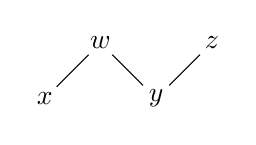
\begin{tikzpicture}
    % First, locate each of the nodes and name them
    \node (top) at (0,0) {$w$};
    \node [below left  of=top] (left)  {$x$};
    \node [below right of=top] (bottom right) {$y$};
    \node [above right of=bottom right] (right) {$z$};

    % Now draw the lines:
    \draw [shorten <=-2pt, shorten >=-2pt] (top) -- (left);
    \draw [shorten <=-2pt, shorten >=-2pt] (top) -- (bottom right);
    \draw [shorten <=-2pt, shorten >=-2pt] (bottom right) -- (right);
\end{tikzpicture}

Let's consider two possible cases. Suppose first $w\sim y$, and $x$ and $z$ are only $\sim$ with themselves. Then in order to collapse $\leq$ under $\sim$, we will need $x \leq w\sim y \leq z$ for transitivity. 

Consider next the case that $w\sim y$ and $x\sim z$. In order to collapse this, we will need that $w\sim x\sim y \sim z$.

These examples show that not every equivalence relation can collapse a poset into a poset (even if it only collapses a chain). 

Note that neither of the above problems are possible with {\bf totality}. It seems that what makes the most sense is collapsing by some equivalence relation, and then extending both the ordering and the equivalence relation to generate a legitimate poset. We can explore this later if needed. 



\section{Other notes}

Fineness may also capture the concept of physical dimension. In fact, two description of the same units are ``finitely comparable'' in the sense that one gives a finer description of the other of a finite factor. Descriptions of different unites are either ``infinitely comparable'' (i.e. areas are always bigger than lengths) or not comparable (i.e. position and momentum). Take phase space, points should be comparables and in fact should be equigranular $\eqgran$ so that we can compare sets of finite points. Areas are also comparable to each other, and are comparable to points. However, vertical lines (i.e. ranges in momentum alone) are not comparable to horizontal lines (i.e. ranges in position alone). Symplectic geometry, in fact, gives a size to areas and not to lines.


\bibliographystyle{plain}
\bibliography{bibliography}

\end{document}
